%% ============================================================
%%  CHAPTER 8 — FEATURE EXTRACTION
%% ============================================================
\chapter{Feature Extraction}
\label{ch:feature_extraction}

This chapter describes the channel-aware, physiologically
motivated feature extraction scheme that transforms each
preprocessed \acrshort{eeg} epoch into a 93-dimensional
feature vector --- the base superset from which every stage of
the classification architecture in Chapter~9 draws its inputs.
Section~\ref{sec:fe_overview} provides an
overview of the feature extraction design philosophy.
Section~\ref{sec:fe_groups} defines the channel groups used
and their physiological justification. Section~\ref{sec:fe_time}
describes time-domain features. Section~\ref{sec:fe_freq}
describes frequency-domain features. Section~\ref{sec:fe_peak}
describes peak detection features specific to blink
classification. Section~\ref{sec:fe_asym} derives the T3--T4
lateral asymmetry index for bruxism discrimination.
Section~\ref{sec:fe_global} describes global statistical
features. Section~\ref{sec:fe_summary_table} presents the
complete 93-feature inventory. Section~\ref{sec:fe_selection}
describes the SelectKBest feature selection analysis.
Section~\ref{sec:fe_negative} documents a set of extended
feature engineering experiments --- wavelet, energy-operator,
and EMG-descriptor features --- most of which \emph{failed} to
improve on the base superset, and explains why those failures
were diagnostically important rather than simply negative
results. Section~\ref{sec:fe_summary} summarises the chapter.

%% ----------------------------------------------------------
\section{Feature Extraction Design Philosophy}
\label{sec:fe_overview}
%% ----------------------------------------------------------

The feature extraction scheme in this project departs from the
standard \acrshort{bci} approach of applying a single feature
type uniformly across all channels (such as \acrshort{csp}
log-variance). Instead, a \textit{channel-aware} approach is
adopted: different feature sets are extracted from different
electrode groups, chosen specifically for their physiological
relevance to the artifact types being classified.

This design is motivated by the observation that the five
artifact classes produce spatially localised signals:

\begin{itemize}[leftmargin=*]
    \item Blink artifacts are dominated by large-amplitude
    deflections at \textbf{frontal} electrodes (Fp1, Fp2).
    \item Jaw artifacts (clinch and bruxism) are dominated by
    broadband \acrshort{emg} contamination at \textbf{temporal}
    electrodes (T3, T4).
    \item Left/right bruxism discrimination requires comparing
    the \textbf{asymmetry} between T3 and T4.
    \item Global statistical properties (kurtosis, skewness)
    that characterise the non-Gaussian distribution of artifact
    signals are best computed over \textbf{all} channels.
\end{itemize}

Applying \acrshort{csp} to this problem would be suboptimal
because \acrshort{csp} is designed for two-class problems and
seeks global spatial filters that maximise variance differences
— it does not exploit the known localisation of the artifact
signals or the asymmetry between T3 and T4.

Figure~\ref{fig:feature_overview} illustrates the feature
extraction architecture.

\begin{figure}[htbp]
\centering
\begin{tikzpicture}[
    node distance=0.4cm and 0.3cm,
    box/.style={rectangle, rounded corners=3pt, draw=black,
                minimum width=3.8cm, minimum height=0.75cm,
                align=center, font=\small},
    arrow/.style={-{Stealth[length=5pt]}, thick},
    group/.style={rectangle, rounded corners=5pt, draw=black,
                  dashed, inner sep=6pt}
]

%% Input epoch
\node[box, fill=green!15, minimum width=8cm]
    (epoch) {Preprocessed Epoch
             $\mathbf{E} \in \mathbb{R}^{19 \times 400}$};

%% Three branches
\node[box, fill=blue!15, below left=0.8cm and 1.5cm of epoch]
    (frontal) {Frontal Group\\Fp1, Fp2};
\node[box, fill=orange!20, below=0.8cm of epoch]
    (temporal) {Temporal Group\\T3, T4};
\node[box, fill=purple!15, below right=0.8cm and 1.5cm of epoch]
    (global) {All 19 Channels};

%% Feature boxes
\node[box, fill=blue!10, below=0.4cm of frontal, minimum width=3.8cm]
    (f_feat) {Time-domain\\Band power\\Peak features};
\node[box, fill=orange!10, below=0.4cm of temporal, minimum width=3.8cm]
    (t_feat) {Time-domain\\Band power\\Asymmetry index};
\node[box, fill=purple!10, below=0.4cm of global, minimum width=3.8cm]
    (g_feat) {Kurtosis\\Skewness};

%% Feature counts
\node[font=\scriptsize\bfseries, blue!70, below=0.1cm of f_feat]
    {(38 features)};
\node[font=\scriptsize\bfseries, orange!80!black, below=0.1cm of t_feat]
    {(36 features)};
\node[font=\scriptsize\bfseries, purple!70, below=0.1cm of g_feat]
    {(19 features)};

%% Concatenation
\node[box, fill=red!10, minimum width=9cm,
      below=1.5cm of t_feat]
    (concat) {Feature Vector Concatenation:
              $\mathbf{f} \in \mathbb{R}^{93}$};

%% Arrows from epoch to groups
\draw[arrow] (epoch.south) -| (frontal.north);
\draw[arrow] (epoch.south) -- (temporal.north);
\draw[arrow] (epoch.south) -| (global.north);

%% Arrows from groups to features
\draw[arrow] (frontal)  -- (f_feat);
\draw[arrow] (temporal) -- (t_feat);
\draw[arrow] (global)   -- (g_feat);

%% Arrows to concat
\draw[arrow] (f_feat.south) |- (concat.west);
\draw[arrow] (t_feat.south) -- (concat.north);
\draw[arrow] (g_feat.south) |- (concat.east);

\end{tikzpicture}
\caption{Feature extraction architecture. The preprocessed
epoch is divided into three channel groups, each producing a
physiologically motivated feature subset. The three subsets
are concatenated into a 93-dimensional feature vector.}
\label{fig:feature_overview}
\end{figure}

%% ----------------------------------------------------------
\section{Channel Groups and Physiological Justification}
\label{sec:fe_groups}
%% ----------------------------------------------------------

Table~\ref{tab:channel_groups} defines the three channel
groups used in feature extraction and the artifact types
each group is designed to characterise.

\begin{table}[htbp]
\centering
\caption{Channel groups used in feature extraction with their
physiological roles and feature counts.}
\label{tab:channel_groups}
\renewcommand{\arraystretch}{1.3}
\begin{tabular}{p{2.2cm} p{2.5cm} p{3.5cm} c}
\toprule
\textbf{Group} & \textbf{Channels} & \textbf{Target Artifact} &
\textbf{Features} \\
\midrule
Frontal  & Fp1, Fp2            & Eye blinks (single, double) & 38 \\
Temporal & T3, T4              & Jaw clinch, bruxism (L/R) & 36 \\
Global   & All 19 channels     & Class-discriminating statistics & 19 \\
\midrule
\textbf{Total} & & & \textbf{93} \\
\bottomrule
\end{tabular}
\end{table}

\subsection{Frontal Group (Fp1, Fp2)}

The frontal polar electrodes Fp1 and Fp2 are positioned
directly above the eyebrows, making them the closest scalp
electrodes to the primary sources of blink artifact: the
corneoretinal potential and the orbicularis oculi muscle.
Blink artifacts at Fp1 and Fp2 are characterised by:

\begin{itemize}[leftmargin=*]
    \item Large amplitude (50--300\,\si{\micro\volt}
    peak-to-peak after bandpass filtering)
    \item Characteristic waveform shape (single or double
    peaks depending on blink count)
    \item Bilateral symmetry (approximately equal at Fp1
    and Fp2 for central blinks)
    \item Slow temporal envelope (peak duration 150--400\,ms
    per blink cycle)
\end{itemize}

Features extracted from Fp1 and Fp2 capture the amplitude,
timing, shape, and spectral content of blink events within
the 2\,s epoch window.

\subsection{Temporal Group (T3, T4)}

The temporal electrodes T3 and T4 overlie the masseter and
temporalis muscles, which are the primary muscles activated
during jaw clinching and bruxism. Jaw artifact signals at
T3 and T4 are characterised by:

\begin{itemize}[leftmargin=*]
    \item Broadband high-frequency content
    (30--80\,Hz \acrshort{emg} energy)
    \item Bilateral activation during clinch (T3
    $\approx$ T4)
    \item Lateralised activation during bruxism
    (T3 $>$ T4 for left, T4 $>$ T3 for right)
    \item Higher amplitude than blink signals
    at these sites (20--100\,\si{\micro\volt} RMS
    after bandpass filtering)
\end{itemize}

Features extracted from T3 and T4 include both individual
channel descriptors and the lateral asymmetry index between
the two channels.

\subsection{Global Group (All 19 Channels)}

Global statistical features — kurtosis and skewness — are
computed across all 19 channels. These features characterise
the non-Gaussian distributional properties of the epoch:

\begin{itemize}[leftmargin=*]
    \item \textbf{Kurtosis} measures the heaviness of the
    distribution tails relative to a Gaussian distribution.
    Artifact epochs (large transient peaks) have much higher
    kurtosis than background \acrshort{eeg}.
    \item \textbf{Skewness} measures the asymmetry of the
    amplitude distribution. Blink artifacts produce
    predominantly positive or negative deflections, resulting
    in non-zero skewness.
\end{itemize}

%% ----------------------------------------------------------
\section{Time-Domain Features}
\label{sec:fe_time}
%% ----------------------------------------------------------

Time-domain features are computed independently for each
channel within the Frontal and Temporal groups. For a single
channel signal $\mathbf{x} = [x_1, x_2, \ldots, x_W]$ with
$W = 400$ samples:

\subsection{Root Mean Square Amplitude}

The \acrfull{rms} amplitude measures the average signal power
within the epoch:

\begin{equation}
\text{RMS}(\mathbf{x}) = \sqrt{\frac{1}{W}
\sum_{t=1}^{W} x_t^2}
\label{eq:rms}
\end{equation}

\acrshort{rms} is the primary indicator of gesture activity.
Blink and jaw artifact epochs have significantly higher
\acrshort{rms} than background \acrshort{eeg} epochs at
their respective electrode sites.

\subsection{Peak-to-Peak Amplitude}

The \acrfull{ptp} amplitude measures the range of the signal:

\begin{equation}
\text{PTP}(\mathbf{x}) = \max(\mathbf{x}) - \min(\mathbf{x})
\label{eq:ptp}
\end{equation}

\acrshort{ptp} is sensitive to the maximum deflection
amplitude of an artifact event. It is particularly
discriminative for blink detection, where the sharp
corneoretinal deflection produces a characteristic spike
in the \acrshort{ptp} value.

\subsection{Zero-Crossing Rate}

The zero-crossing rate measures the frequency of sign changes
in the signal:

\begin{equation}
\text{ZCR}(\mathbf{x}) = \frac{1}{W-1}
\sum_{t=1}^{W-1} \mathbf{1}\left[x_t \cdot x_{t+1} < 0\right]
\label{eq:zcr}
\end{equation}

\noindent where $\mathbf{1}[\cdot]$ is the indicator function.
\acrshort{zcr} is related to the dominant frequency of the
signal: high-frequency \acrshort{emg} (bruxism, clinch) produces
a high \acrshort{zcr}, while slow blink deflections produce
a low \acrshort{zcr}.

\subsection{Hjorth Parameters}

Hjorth parameters~\cite{hjorth1970eeg} provide a compact
characterisation of signal dynamics through three
complementary descriptors. Let $\mathbf{x}' = [x_2 - x_1,
x_3 - x_2, \ldots, x_W - x_{W-1}]$ denote the first
difference (discrete derivative) of $\mathbf{x}$, and
$\mathbf{x}''$ the second difference.

\textbf{Hjorth Activity} is the signal variance:
\begin{equation}
H_A(\mathbf{x}) = \text{var}(\mathbf{x})
= \frac{1}{W}\sum_{t=1}^{W}(x_t - \bar{x})^2
\label{eq:hjorth_activity}
\end{equation}

\textbf{Hjorth Mobility} is the ratio of the standard
deviation of the first derivative to that of the signal,
proportional to the mean frequency:
\begin{equation}
H_M(\mathbf{x}) = \sqrt{\frac{\text{var}(\mathbf{x}')}
{\text{var}(\mathbf{x})}}
\label{eq:hjorth_mobility}
\end{equation}

\textbf{Hjorth Complexity} describes how the shape of the
signal differs from a pure sinusoid:
\begin{equation}
H_C(\mathbf{x}) = \frac{H_M(\mathbf{x}')}
{H_M(\mathbf{x})}
= \frac{\sqrt{\text{var}(\mathbf{x}'')/
\text{var}(\mathbf{x}')}}
{\sqrt{\text{var}(\mathbf{x}')/\text{var}(\mathbf{x})}}
\label{eq:hjorth_complexity}
\end{equation}

Hjorth parameters are amplitude-scale-invariant when combined
with Z-score normalisation, making them robust to inter-session
amplitude differences.

\subsection{Time-Domain Feature Count per Group}

For the Frontal group (2 channels: Fp1, Fp2), the following
time-domain features are extracted per channel:
\{RMS, PTP, ZCR, $H_A$, $H_M$, $H_C$\} = 6 features
$\times$ 2 channels = \textbf{12 features}.

For the Temporal group (2 channels: T3, T4), the same
6 features per channel = \textbf{12 features}.

%% ----------------------------------------------------------
\section{Frequency-Domain Features}
\label{sec:fe_freq}
%% ----------------------------------------------------------

\subsection{Power Spectral Density Estimation}

Frequency-domain features are computed from the Power
Spectral Density (\acrshort{psd}) of each channel signal.
The \acrshort{psd} is estimated using Welch's method with
a Hann window of length 100 samples (0.5\,s) and 50\%
overlap:

\begin{equation}
\hat{P}(f) = \frac{1}{K} \sum_{k=0}^{K-1}
\left|\text{DFT}\{w(t) \cdot x(t + k\Delta)\}\right|^2
\label{eq:welch}
\end{equation}

\noindent where $w(t)$ is the Hann window, $\Delta$ is the
step between windows, and $K$ is the number of windows.
Welch's method reduces variance in the \acrshort{psd}
estimate compared to a single periodogram, at the cost of
frequency resolution — acceptable here since features are
integrated over broad frequency bands.

\subsection{Absolute Band Power}

For each frequency band $[f_l, f_h]$, the absolute band
power is computed by integrating the \acrshort{psd} over
the band:

\begin{equation}
P_{[f_l, f_h]}(\mathbf{x}) =
\int_{f_l}^{f_h} \hat{P}(f)\, df
\approx \sum_{f_k \in [f_l, f_h]} \hat{P}(f_k) \cdot \Delta f
\label{eq:bandpower}
\end{equation}

Five standard \acrshort{eeg} frequency bands are used:

\begin{table}[htbp]
\centering
\caption{EEG frequency bands used for band power feature
extraction.}
\label{tab:freq_bands}
\renewcommand{\arraystretch}{1.3}
\begin{tabular}{llp{5cm}}
\toprule
\textbf{Band} & \textbf{Range (Hz)} & \textbf{Relevance} \\
\midrule
Delta & 0.5 -- 4\,Hz  & Slow blink waveform components \\
Theta & 4 -- 8\,Hz    & Transition band, general EEG activity \\
Alpha & 8 -- 13\,Hz   & Background EEG, suppressed during activity \\
Beta  & 13 -- 30\,Hz  & Bruxism EMG onset, motor activity \\
Gamma & 30 -- 45\,Hz  & High-frequency jaw EMG (primary bruxism
                        discriminator) \\
\bottomrule
\end{tabular}
\end{table}

\subsection{Relative Band Power}

In addition to absolute band power, the relative band power
is computed for each band as the fraction of total power:

\begin{equation}
P^{\text{rel}}_{[f_l,f_h]}(\mathbf{x}) =
\frac{P_{[f_l,f_h]}(\mathbf{x})}
{\sum_b P_b(\mathbf{x})}
\label{eq:rel_bandpower}
\end{equation}

\noindent where the sum in the denominator is over all five
bands. Relative band power is dimensionless and amplitude-
invariant — it captures the \textit{spectral shape} of the
signal rather than its absolute energy level. This property
makes it robust to inter-session amplitude differences that
are not fully corrected by Z-score normalisation.

\subsection{Frequency-Domain Feature Count per Group}

For each channel in the Frontal and Temporal groups, 5
absolute band power features and 5 relative band power
features are extracted = 10 features per channel.

\begin{itemize}[leftmargin=*]
    \item Frontal group (Fp1, Fp2): 10 features
    $\times$ 2 channels = \textbf{20 features}
    \item Temporal group (T3, T4): 10 features
    $\times$ 2 channels = \textbf{20 features}
\end{itemize}

\subsection{Key Discriminative Band: Gamma Power at T4}

The SelectKBest analysis (Section~\ref{sec:fe_selection})
identifies T4 gamma power as the single most discriminative
feature in the entire 93-feature vector. This is because
gamma-band \acrshort{emg} power at T4 is strongly elevated
during right bruxism and jaw clinch but remains low during
blink events and rest — providing near-perfect discrimination
between the two major signal families (ocular vs.\ jaw
artifacts).

%% ----------------------------------------------------------
\section{Peak Detection Features}
\label{sec:fe_peak}
%% ----------------------------------------------------------

Peak detection features are extracted exclusively from the
Frontal group (Fp1, Fp2) and are designed to discriminate
between single and double blinks based on the number and
timing of deflection peaks within the epoch window.

\subsection{Peak Count}

The number of local maxima exceeding a prominence threshold
$\theta_p$ in the \acrshort{ptp}-normalised frontal signal:

\begin{equation}
N_{\text{peaks}} = \left|\left\{t : x(t) \text{ is a local
maximum and } x(t) > \theta_p \cdot \text{PTP}(x)\right\}\right|
\label{eq:peak_count}
\end{equation}

The threshold $\theta_p = 0.3$ (30\% of the epoch
peak-to-peak range) prevents noise fluctuations from being
counted as peaks. $N_{\text{peaks}}$ is designed to directly
encode the blink count: nominally 1 for a single blink, 2 for
a double blink.

\textbf{Important caveat:} this peak-counting approach assumes
that a recording labelled ``single blink'' actually contains a
single, isolated blink. As documented in Chapter~6, roughly
45\% of \code{single\_blink} recordings actually contain a
cluster of three or more blinks, which $N_{\text{peaks}}$
would count as 3 or more --- i.e., the feature itself is
computed correctly, but the underlying assumption that the
count reflects the intended class breaks down for a substantial
fraction of the data. This is precisely why counting-based
features, however carefully engineered, could not resolve the
final blink sub-classification on their own; four
counting-based variants (of which $N_{\text{peaks}}$ is one)
were tried and rejected during classifier development, in
favour of the waveform shape-matching approach described in
Chapter~9.

\subsection{Peak Interval}

The mean time interval between consecutive detected peaks:

\begin{equation}
\bar{\Delta t}_{\text{peaks}} = \frac{1}{N_{\text{peaks}}-1}
\sum_{k=1}^{N_{\text{peaks}}-1} (t_{k+1} - t_k)
\label{eq:peak_interval}
\end{equation}

\noindent set to zero when $N_{\text{peaks}} \leq 1$.
The peak interval is designed to characterise the timing of a
double blink (inter-blink interval $\approx$200--400\,ms),
though its reliability is subject to the same contamination
caveat noted above.

\subsection{Peak Amplitude Statistics}

The mean and standard deviation of detected peak amplitudes:

\begin{align}
\bar{A}_{\text{peaks}} &= \frac{1}{N_{\text{peaks}}}
\sum_{k=1}^{N_{\text{peaks}}} x(t_k)
\label{eq:peak_mean} \\
\sigma_{A,\text{peaks}} &= \sqrt{\frac{1}{N_{\text{peaks}}}
\sum_{k=1}^{N_{\text{peaks}}}
\left(x(t_k) - \bar{A}_{\text{peaks}}\right)^2}
\label{eq:peak_std}
\end{align}

\subsection{Peak Feature Count}

Peak features are computed for each of the 2 frontal channels
(Fp1, Fp2): \{$N_{\text{peaks}}$, $\bar{\Delta t}$,
$\bar{A}$, $\sigma_A$\} = 4 features $\times$ 2 channels
= \textbf{6 features} from peak detection (the remaining
2 features per channel are inter-channel peak correlation and
peak symmetry between Fp1 and Fp2).

Total frontal features: 12 (time-domain) + 20 (frequency)
+ 6 (peak) = \textbf{38 features}.

%% ----------------------------------------------------------
\section{T3--T4 Lateral Asymmetry Index}
\label{sec:fe_asym}
%% ----------------------------------------------------------

The lateral asymmetry index is the key feature for
discriminating between left and right bruxism. Without this
feature, the classifier cannot distinguish the two bruxism
classes because both produce high \acrshort{emg} energy at
the temporal sites — the only difference is which side
is dominant.

\subsection{Derivation}

Let $A_{T3}$ and $A_{T4}$ denote the \acrshort{rms}
amplitudes of channels T3 and T4 within epoch $\mathbf{E}_k$:

\begin{align}
A_{T3} &= \text{RMS}\left(\mathbf{E}_k[T3, :]\right) \\
A_{T4} &= \text{RMS}\left(\mathbf{E}_k[T4, :]\right)
\end{align}

The normalised asymmetry index is defined as:

\begin{equation}
\boxed{
\mathcal{A}_{T3,T4} = \frac{A_{T4} - A_{T3}}
{A_{T4} + A_{T3} + \epsilon}
}
\label{eq:asymmetry}
\end{equation}

\noindent where $\epsilon = 10^{-8}$ prevents division by
zero. The normalisation by the sum of both amplitudes ensures
that the index is bounded in the interval $(-1, +1)$,
making it invariant to the absolute amplitude of the jaw
\acrshort{emg} signal.

\subsection{Interpretation}

\begin{itemize}[leftmargin=*]
    \item $\mathcal{A}_{T3,T4} > 0$: T4 dominant
    $\rightarrow$ \textbf{Right bruxism}
    \item $\mathcal{A}_{T3,T4} < 0$: T3 dominant
    $\rightarrow$ \textbf{Left bruxism}
    \item $\mathcal{A}_{T3,T4} \approx 0$: Bilateral
    $\rightarrow$ \textbf{Jaw clinch}
\end{itemize}

This three-way separation is illustrated in
Figure~\ref{fig:asymmetry}.

\begin{figure}[htbp]
\centering
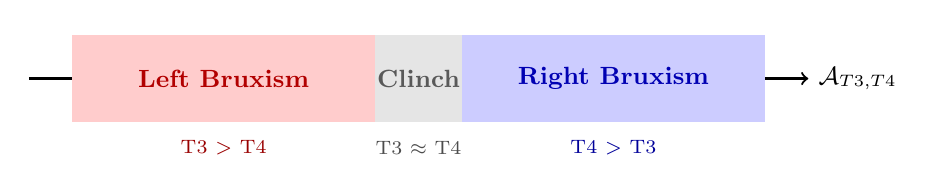
\begin{tikzpicture}[scale=1.1]
    %% Number line
    \draw[thick, ->] (-4.5,0) -- (4.5,0)
        node[right]{\small $\mathcal{A}_{T3,T4}$};
    \draw[thick] (0,-0.15) -- (0,0.15)
        node[above]{\small 0};
    \draw[thick] (-3,-0.15) -- (-3,0.15)
        node[above]{\small $-$1};
    \draw[thick] (3,-0.15) -- (3,0.15)
        node[above]{\small $+$1};

    %% Regions
    \fill[red!20]    (-4.0,-0.5) rectangle (-0.5, 0.5);
    \fill[gray!20]   (-0.5,-0.5) rectangle ( 0.5, 0.5);
    \fill[blue!20]   ( 0.5,-0.5) rectangle ( 4.0, 0.5);

    %% Labels
    \node[font=\small\bfseries, red!70!black]
        at (-2.25, 0) {Left Bruxism};
    \node[font=\small\bfseries, gray!70!black]
        at (0, 0) {Clinch};
    \node[font=\small\bfseries, blue!70!black]
        at (2.25, 0) {Right Bruxism};

    %% Sub-labels
    \node[font=\scriptsize, red!60!black]
        at (-2.25, -0.8) {T3 $>$ T4};
    \node[font=\scriptsize, gray!60!black]
        at (0, -0.8) {T3 $\approx$ T4};
    \node[font=\scriptsize, blue!60!black]
        at (2.25, -0.8) {T4 $>$ T3};
\end{tikzpicture}
\caption{Interpretation of the T3--T4 normalised asymmetry
index $\mathcal{A}_{T3,T4}$. Left bruxism produces T3
dominance (negative index), jaw clinch produces bilateral
activation (near-zero index), and right bruxism produces
T4 dominance (positive index). This index improved
bruxism\_left F1 from 0.609 to 0.737 (+0.128).}
\label{fig:asymmetry}
\end{figure}

\subsection{Band-Specific Asymmetry}

In addition to the broadband \acrshort{rms} asymmetry index,
asymmetry indices are computed separately for the beta and
gamma band \acrshort{rms} amplitudes at T3 and T4, providing
three asymmetry features in total:

\begin{align}
\mathcal{A}^{\text{broad}} &= \frac{A_{T4}^{\text{broad}}
- A_{T3}^{\text{broad}}}{A_{T4}^{\text{broad}}
+ A_{T3}^{\text{broad}} + \epsilon} \\
\mathcal{A}^{\text{beta}} &= \frac{A_{T4}^{\text{beta}}
- A_{T3}^{\text{beta}}}{A_{T4}^{\text{beta}}
+ A_{T3}^{\text{beta}} + \epsilon} \\
\mathcal{A}^{\text{gamma}} &= \frac{A_{T4}^{\text{gamma}}
- A_{T3}^{\text{gamma}}}{A_{T4}^{\text{gamma}}
+ A_{T3}^{\text{gamma}} + \epsilon}
\end{align}

These three asymmetry features are appended to the Temporal
group feature vector, bringing the total temporal features to:
12 (time-domain) + 20 (frequency-domain) + 3 (asymmetry)
+ 1 (clinch indicator) = \textbf{36 features}.

%% ----------------------------------------------------------
\section{Global Statistical Features}
\label{sec:fe_global}
%% ----------------------------------------------------------

Global statistical features are computed independently for
each of the 19 channels from the epoch signal after
Z-score normalisation.

\subsection{Kurtosis}

Kurtosis measures the heaviness of the tails of the
amplitude distribution relative to a Gaussian (which has
kurtosis = 3). The excess kurtosis is:

\begin{equation}
\kappa(\mathbf{x}) = \frac{\frac{1}{W}\sum_{t=1}^{W}
(x_t - \bar{x})^4}{\left(\frac{1}{W}\sum_{t=1}^{W}
(x_t - \bar{x})^2\right)^2} - 3
\label{eq:kurtosis}
\end{equation}

Artifact epochs containing large transient deflections have
high kurtosis (heavy tails), while rest \acrshort{eeg}
epochs have near-Gaussian distributions (kurtosis
$\approx$ 0). Kurtosis thus serves as a global measure of
artifact presence across all channels, complementing the
localised \acrshort{rms} features of the frontal and
temporal groups.

\subsection{Skewness}

Skewness measures the asymmetry of the amplitude
distribution:

\begin{equation}
\gamma(\mathbf{x}) = \frac{\frac{1}{W}\sum_{t=1}^{W}
(x_t - \bar{x})^3}{\left(\frac{1}{W}\sum_{t=1}^{W}
(x_t - \bar{x})^2\right)^{3/2}}
\label{eq:skewness}
\end{equation}

Blink artifacts produce predominantly unipolar deflections
(positive or negative), resulting in non-zero skewness.
Bilateral jaw artifacts tend to produce more symmetric
deflections (near-zero skewness at most channels, with
strong skewness at T3 or T4 depending on laterality).

\subsection{Global Feature Count}

One kurtosis and one skewness value per channel:
2 features $\times$ 19 channels = \textbf{38 features}.

However, only kurtosis is used as a global feature (one
per channel = 19 features), with skewness reserved for
the frontal and temporal groups where it has the highest
discriminative value. Global feature total: \textbf{19
features}.

%% ----------------------------------------------------------
\section{Complete Feature Vector}
\label{sec:fe_summary_table}
%% ----------------------------------------------------------

Table~\ref{tab:feature_inventory} provides the complete
inventory of all 93 features organised by group.

\begin{table}[htbp]
\centering
\caption{Complete 93-feature inventory organised by channel
group. Features are computed per channel within each group
unless otherwise stated.}
\label{tab:feature_inventory}
\renewcommand{\arraystretch}{1.25}
\begin{tabular}{p{1.5cm} p{2.5cm} p{4.0cm} c}
\toprule
\textbf{Group} & \textbf{Channels} & \textbf{Feature} &
\textbf{Count} \\
\midrule
\multirow{6}{*}{Frontal}
 & \multirow{6}{*}{Fp1, Fp2}
 & RMS amplitude                    & 2 \\
 & & Peak-to-peak amplitude         & 2 \\
 & & Zero-crossing rate             & 2 \\
 & & Hjorth activity                & 2 \\
 & & Hjorth mobility                & 2 \\
 & & Hjorth complexity              & 2 \\
 & & Delta band power (abs.)        & 2 \\
 & & Theta band power (abs.)        & 2 \\
 & & Alpha band power (abs.)        & 2 \\
 & & Beta band power (abs.)         & 2 \\
 & & Gamma band power (abs.)        & 2 \\
 & & Delta band power (rel.)        & 2 \\
 & & Theta band power (rel.)        & 2 \\
 & & Alpha band power (rel.)        & 2 \\
 & & Beta band power (rel.)         & 2 \\
 & & Gamma band power (rel.)        & 2 \\
 & & Peak count                     & 2 \\
 & & Mean peak interval             & 2 \\
 & & Mean peak amplitude            & 2 \\
\multirow{1}{*}{}
 & & \textit{Frontal subtotal}      & \textbf{38} \\
\midrule
\multirow{6}{*}{Temporal}
 & \multirow{6}{*}{T3, T4}
 & RMS amplitude                    & 2 \\
 & & Peak-to-peak amplitude         & 2 \\
 & & Zero-crossing rate             & 2 \\
 & & Hjorth activity                & 2 \\
 & & Hjorth mobility                & 2 \\
 & & Hjorth complexity              & 2 \\
 & & Delta band power (abs.)        & 2 \\
 & & Theta band power (abs.)        & 2 \\
 & & Alpha band power (abs.)        & 2 \\
 & & Beta band power (abs.)         & 2 \\
 & & Gamma band power (abs.)        & 2 \\
 & & Delta band power (rel.)        & 2 \\
 & & Theta band power (rel.)        & 2 \\
 & & Alpha band power (rel.)        & 2 \\
 & & Beta band power (rel.)         & 2 \\
 & & Gamma band power (rel.)        & 2 \\
 & & Asymmetry index (broadband)    & 1 \\
 & & Asymmetry index (beta)         & 1 \\
 & & Asymmetry index (gamma)        & 1 \\
\multirow{1}{*}{}
 & & \textit{Temporal subtotal}     & \textbf{36} \\
\midrule
Global
 & All 19 ch
 & Kurtosis (per channel)          & 19 \\
 & & \textit{Global subtotal}      & \textbf{19} \\
\midrule
\multicolumn{3}{r}{\textbf{Total features}} & \textbf{93} \\
\bottomrule
\end{tabular}
\end{table}

%% ----------------------------------------------------------
\section{Feature Selection: SelectKBest Analysis}
\label{sec:fe_selection}
%% ----------------------------------------------------------

\subsection{Motivation}

Although 93 features is a relatively compact vector for a
machine learning classifier with 1{,}246 activity-gated
training samples (Chapter~6; sample-to-feature ratio
$\approx 13.4:1$, above the 10:1 rule of thumb for stable
classification, though less comfortably so than in the earlier
2-session dataset), a feature
selection analysis was conducted to (a) verify that the
engineered features contain genuine discriminative information,
(b) identify which features contribute most to classification,
and (c) guide future feature set refinement.

\subsection{Method}

The SelectKBest algorithm with mutual information scoring
was applied to rank all 93 features by their univariate
association with the class label. Mutual information
$I(X; Y)$ between a feature $X$ and the class label $Y$
measures the reduction in uncertainty about $Y$ given
knowledge of $X$:

\begin{equation}
I(X; Y) = \sum_{x, y} p(x, y) \log
\frac{p(x, y)}{p(x)\,p(y)}
\label{eq:mutual_info}
\end{equation}

Unlike correlation-based scoring, mutual information
captures nonlinear associations and is therefore appropriate
for the mixed feature types in this feature vector.

\subsection{Top Features}

Table~\ref{tab:top_features} lists the top 10 features by
mutual information score.

\begin{table}[htbp]
\centering
\caption{Top 10 features ranked by mutual information score
with the class label. All top features are from the frontal
or temporal channel groups, confirming the physiological
relevance of the channel-aware design.}
\label{tab:top_features}
\renewcommand{\arraystretch}{1.3}
\begin{tabular}{c p{4.5cm} p{3.0cm}}
\toprule
\textbf{Rank} & \textbf{Feature} & \textbf{Discriminates} \\
\midrule
1  & T4 gamma band power (abs.)    & Jaw vs.\ blink \\
2  & T4 peak-to-peak amplitude     & Jaw EMG amplitude \\
3  & T4 beta band power (abs.)     & Bruxism pattern \\
4  & Fp1 peak-to-peak amplitude    & Blink amplitude \\
5  & Fp2 peak-to-peak amplitude    & Blink amplitude \\
6  & T3--T4 asymmetry (broadband)  & L vs.\ R bruxism \\
7  & T4 gamma band power (rel.)    & Jaw spectral shape \\
8  & T3 gamma band power (abs.)    & Jaw bilateral \\
9  & Fp1 peak count                & Blink count (1/2) \\
10 & Fp2 peak count                & Blink count (1/2) \\
\bottomrule
\end{tabular}
\end{table}

The top 10 features confirm the design rationale:

\begin{itemize}[leftmargin=*]
    \item \textbf{Ranks 1--3:} T4 features dominate because
    T4 gamma power is the strongest single discriminator
    between jaw artifact classes (clinch/bruxism) and blink
    classes — the primary inter-class boundary in the dataset.
    \item \textbf{Ranks 4--5:} Fp1/Fp2 \acrshort{ptp} is
    the primary blink indicator — high for any blink type,
    low for jaw artifacts and rest.
    \item \textbf{Rank 6:} The T3--T4 asymmetry index is
    ranked 6th globally, confirming its importance for
    bruxism lateralisation without being the top feature
    (because it is only discriminative within the jaw
    artifact family, not across all five classes).
    \item \textbf{Ranks 9--10:} Peak count at Fp1/Fp2
    directly encodes the blink count and is, on paper,
    discriminative for single vs.\ double blink
    classification --- though as noted in
    Section~\ref{sec:fe_peak}, this univariate ranking does
    not capture the contamination problem diagnosed in
    Chapter~6, which is why the final blink sub-classifier
    (Chapter~9) does not rely on peak count alone.
\end{itemize}

\subsection{Feature Retention Decision}

All 93 features were retained for the baseline flat classifier
(no feature selection was applied at training time). This
decision was made because:

\begin{enumerate}[leftmargin=*]
    \item The sample-to-feature ratio ($\approx$13.4:1) is
    adequate for Random Forest, which handles irrelevant
    features well through its internal random feature
    subsampling at each split.
    \item Removing features based on univariate mutual
    information ignores feature interactions, which may
    be important for multi-class discrimination.
    \item The SelectKBest analysis confirmed that all
    feature groups contain at least some discriminative
    features (no group is entirely uninformative).
\end{enumerate}

This 93-feature retention policy applies to the \emph{flat}
baseline model specifically. The final hybrid architecture
(Chapter~9) does not use all 93 features identically at every
stage: it extracts a superset once (93 base features, extended
to 129 once the EMG descriptors introduced in
Section~\ref{sec:fe_negative} are included), and each stage of
the hierarchy selects its own relevant columns by name --- the
blink/muscle router uses frontal and temporal features
together, the muscle sub-classifier leans on the Riemannian
covariance representation rather than these hand-crafted
features at all, and the blink sub-classifier ultimately uses
the raw waveform directly (\acrshort{dtw}) rather than any
column of this feature vector. Feature selection is therefore
handled architecturally, by routing, rather than by discarding
columns.

%% ----------------------------------------------------------
\section{Extended Feature Engineering Experiments (Negative Results)}
\label{sec:fe_negative}
%% ----------------------------------------------------------

\subsection{Motivation}

Beyond the 93-feature superset described above, a systematic
exploration of more advanced feature families was carried out
in search of further accuracy gains, evaluated under
GroupKFold cross-validation against a 77.2\% baseline (the
93-feature flat classifier). This section documents that
exploration in full, including the experiments that
\textbf{failed}, because the pattern of failure turned out to
be one of the most important diagnostic findings of the
project --- it is what ultimately motivated the hierarchical,
physiology-routed architecture of Chapter~9, rather than a
larger flat feature vector.

\subsection{The Experiments}

Table~\ref{tab:feature_experiments} summarises four extended
feature families that were implemented and tested.

\begin{table}[htbp]
\centering
\caption{Extended feature engineering experiments, evaluated
under GroupKFold against the 93-feature baseline (77.2\%).}
\label{tab:feature_experiments}
\renewcommand{\arraystretch}{1.3}
\begin{tabular}{p{3.3cm} p{3.0cm} p{6.0cm}}
\toprule
\textbf{Feature family} & \textbf{Result vs.\ baseline} &
\textbf{Verdict} \\
\midrule
Discrete Wavelet Transform (full, 108 feats) & $-$14.4\% &
Catastrophic --- amplitude-scaled wavelet coefficients act as
noise rather than signal \\
DWT relative-energy only (36 feats) & break-even ($+$0.1\%) &
Wash --- helps blink classes, costs clinch \\
Teager--Kaiser Energy Operator (\acrshort{tkeo}) & $-$5.7\% &
Squared-amplitude energy measure does not survive cross-session
amplitude drift \\
\acrshort{emg} descriptors (waveform length, slope sign
changes, Willison amplitude, coefficient of variation) &
$-$3.1\% overall, but clinch $+$0.06, bruxism\_left $+$0.06 &
Helps muscle classes specifically, hurts blink classes \\
\bottomrule
\end{tabular}
\end{table}

\subsection{Discrete Wavelet Transform (DWT)}

A full \acrshort{dwt} decomposition (108 features: energy and
statistical moments per sub-band, per channel) was tested as a
richer alternative to Welch band power. It performed
catastrophically ($-$14.4\%): because \acrshort{dwt}
coefficients are not amplitude-normalised the way relative band
power is, they re-introduce exactly the cross-session amplitude
sensitivity that Z-score normalisation and relative band power
were designed to avoid (Chapter~7). A reduced variant using
only relative wavelet sub-band energy (36 features) removed
this sensitivity and came out roughly break-even overall
($+$0.1\%), but the aggregate figure conceals a trade-off: it
helped the blink classes while costing the clinch class,
netting out to no real gain.

\subsection{Teager--Kaiser Energy Operator (TKEO)}

The \acrshort{tkeo} is a classical instantaneous-energy
operator, commonly used in \acrshort{emg} onset detection, of
the form $\Psi[x(t)] = x^2(t) - x(t-1)\,x(t+1)$. It was tested
as a potential improvement over plain \acrshort{rms}/band-power
energy for the jaw \acrshort{emg} classes. It underperformed by
$-$5.7\%. The reason is directly related to the muscle-class
cross-session generalisation problem discussed in Chapter~9:
\acrshort{tkeo}, like \acrshort{dwt}, is a squared-amplitude
measure, and squared-amplitude measures do not survive the
day-to-day amplitude drift between recording sessions. This
negative result is what later motivated trying a
representation that is inherently insensitive to absolute
amplitude --- Riemannian covariance geometry --- for the muscle
branch of the final architecture (Chapter~9).

\subsection{EMG Descriptors (Waveform Length, Slope Sign
Changes, Willison Amplitude, Coefficient of Variation)}

A set of four classical surface-\acrshort{emg} descriptors,
widely used in prosthetics and gesture-recognition literature,
was added to the feature vector: waveform length (cumulative
path length of the signal), slope sign changes (a measure of
frequency content), Willison amplitude (counts of amplitude
changes exceeding a threshold), and coefficient of variation.
Added to the full 93-feature vector, these hurt overall
accuracy by $-$3.1\% on the flat classifier --- but the
aggregate number hides a class-specific split: clinch F1
improved by $+$0.06 and bruxism\_left F1 by $+$0.06, i.e., the
EMG descriptors are genuinely useful for the muscle classes and
actively harmful for the blink classes (which have no
meaningful ``EMG'' content to describe).

\subsection{The Key Realisation}

Every one of these extended feature families showed the same
pattern: discriminative power for \emph{one} class group
(either blink or muscle) while acting as pure noise --- or
worse, active interference --- for the other:

\begin{itemize}[leftmargin=*]
    \item Muscle-oriented features (\acrshort{emg} descriptors,
    \acrshort{tkeo}) help clinch/bruxism but are meaningless
    for blinks, which are frontal \acrshort{eog} events with no
    muscle-fibre recruitment pattern to describe.
    \item A single flat classifier, trained on the concatenation
    of all features across all classes, has no way to apply a
    feature family \emph{conditionally} --- it must either
    include a feature for every class or exclude it for every
    class, even when that feature is only meaningful for half
    the taxonomy.
\end{itemize}

\textbf{The bottleneck was architectural, not feature count.}
This realisation --- that no amount of additional feature
engineering on top of a single flat classifier could resolve
the blink/muscle asymmetry --- is what motivated the
hierarchical, physiology-routed design described in Chapter~9,
in which the EMG descriptors that failed here are reintroduced
specifically for the muscle branch (where they help), while the
blink branch is routed to waveform shape-matching instead of
any hand-crafted feature at all. The 129-feature superset
referenced in Chapter~9 corresponds to the base 93 features
plus these four EMG descriptor families, extracted once and
selected by column per stage rather than applied uniformly.

%% ----------------------------------------------------------
\section{Chapter Summary}
\label{sec:fe_summary}
%% ----------------------------------------------------------

This chapter presented the complete channel-aware feature
extraction scheme producing a 93-dimensional base feature
vector from each preprocessed \acrshort{eeg} epoch. Three
channel groups were defined based on physiological relevance:
the Frontal group (Fp1, Fp2; 38 features) captures blink
morphology through time-domain statistics, band power, and
peak detection features; the Temporal group (T3, T4; 36
features) captures jaw \acrshort{emg} characteristics
through the same feature types plus the T3--T4 normalised
lateral asymmetry index that enables left/right bruxism
discrimination; and the Global group (all 19 channels;
19 features) captures kurtosis across all channels as
a global artifact presence indicator. Full mathematical
derivations were provided for all features including
\acrshort{rms}, \acrshort{ptp}, \acrshort{zcr}, Hjorth
parameters, band power (absolute and relative), peak
detection statistics, and the asymmetry index. A
SelectKBest mutual information analysis confirmed the
physiological relevance of the channel-aware design,
with T4 gamma power, blink peak amplitude, and the
T3--T4 asymmetry index ranking among the top
discriminative features -- while also showing that peak-count
features, though individually well-ranked, are undermined by
the single-blink contamination problem identified in Chapter~6.

Four extended feature families beyond the base superset were
also tested --- full \acrshort{dwt} ($-$14.4\%), relative-energy
\acrshort{dwt} (break-even), \acrshort{tkeo} ($-$5.7\%), and EMG
descriptors ($-$3.1\% overall, but positive specifically for
clinch and bruxism\_left) --- and all four either failed
outright or split sharply between helping the muscle classes
and hurting the blink classes. This consistent pattern showed
that the limitation was architectural rather than a matter of
feature count: a single flat classifier cannot apply a feature
family conditionally to only the classes it is relevant for.
This finding directly motivates the hierarchical, physiology-routed
classification architecture of Chapter~9, which extracts a
129-feature superset (the 93 base features plus the four EMG
descriptor families) and routes different column subsets --
and, for the blink and muscle branches specifically, entirely
different representations (\acrshort{dtw} shape-matching and
Riemannian covariance geometry) -- to each stage rather than
feeding one flat vector to one flat classifier. The following
chapter describes this classification and training methodology
in full.